\documentclass[11pt]{scrartcl}
\newcommand*\student[1]{\newcommand{\thestudent}{{#1}}}



\student{Hun Rim}

%----------------------------------------------------------------------------------------
%	PACKAGES AND OTHER DOCUMENT CONFIGURATIONS
%----------------------------------------------------------------------------------------

\usepackage[utf8]{inputenc} % Required for inputting international characters
\usepackage[T1]{fontenc} % Use 8-bit encoding
\usepackage[sc]{mathpazo}
\usepackage{caption, subcaption}
\usepackage{hyperref}
\usepackage{inconsolata}

\usepackage[english]{babel} % English language hyphenation
\usepackage{amsmath, amsfonts} % Math packages
\usepackage{listings} % Code listings, with syntax highlighting
\usepackage{graphicx} % Required for inserting images
\graphicspath{{Figures/}{./}} % Specifies where to look for included images (trailing slash required)
\usepackage{float}

%----------------------------------------------------------------------------------------
%	DOCUMENT MARGINS
%----------------------------------------------------------------------------------------

\usepackage{geometry} % For page dimensions and margins
\geometry{
	paper=a4paper, 
	top=2.5cm, % Top margin
	bottom=3cm, % Bottom margin
	left=3cm, % Left margin
	right=3cm, % Right margin
}

%----------------------------------------------------------------------------------------
%	SECTION TITLES
%----------------------------------------------------------------------------------------

\usepackage{sectsty}
\sectionfont{\vspace{6pt}\centering\normalfont\scshape}
\subsectionfont{\normalfont\bfseries} % \subsection{} styling
\subsubsectionfont{\normalfont\itshape} % \subsubsection{} styling
\paragraphfont{\normalfont\scshape} % \paragraph{} styling

%----------------------------------------------------------------------------------------
%	HEADERS AND FOOTERS
%----------------------------------------------------------------------------------------

\usepackage{scrlayer-scrpage}
\ofoot*{\pagemark} % Right footer
\ifoot*{\thestudent} % Left footer
\cfoot*{} % Centre footer

%----------------------------------------------------------------------------------------
%	TITLE SECTION
%----------------------------------------------------------------------------------------

\title{	
	\normalfont\normalsize
	\textsc{Machine Learning\\%
	Universit\`a della Svizzera italiana}\\
	\vspace{25pt}
	\rule{\linewidth}{0.5pt}\\
	\vspace{20pt}
	{\huge Assignment 1}\\
	\vspace{12pt}
	\rule{\linewidth}{1pt}\\
	\vspace{12pt}
}

\author{\LARGE \thestudent}

\date{\normalsize\today}

\begin{document}

\maketitle

%The assignment is split into two parts: you are asked to solve a regression problem, and answer some questions. 
%You can use all the books, material, and help you need. 
%Bear in mind that the questions you are asked are similar to those you may find in the final exam, and are related to very important and fundamental machine learning concepts. 
%As such, sooner or later you will need to learn them to pass the course. 
%We will give you some feedback afterwards.\\

\noindent \textbf{!! !!  Note that this file is just meant as a template for the report, in which we reported \textit{part of} the assignment text for convenience. You must always refer to the text in the README.md file as the assignment requirements  !! !!}.

%----------------------------------------------------------------------------------------
%	Tasks
%----------------------------------------------------------------------------------------

\section*{Tasks}

This section should contain a detailed description of how you solved the assignment, including all required statistical analyses of the models' performance and a comparison between the linear regression and the model of your choice. Limit the assignment to 8-10 pages and do not include any code in the report.

\subsection*{Task 1}
Use the family of models $f(\mathbf{x}, \boldsymbol{\theta}) = \theta_0 + \theta_1 \cdot x_1 + \theta_2 \cdot x_2 + \theta_3 \cdot \cos(x_1) + \theta_4 \cdot x_2 \cdot x_2 + \theta_5 \cdot \tanh(x_1)$ to fit the data. 


%theta_0 + theta_1 * x_1 + theta_2 * x_2 + theta_3 * cos(x_1) + theta_4 * x_2 * x_2 + theta_5 * tanh(x_1)

\begin{itemize}
	\item [a.] Write in the report the formula of the model substituting parameters $\theta_0, \ldots, \theta_5$ with the estimates you've found:
	$$f(\mathbf{x}, \boldsymbol{\theta}) =  0.99 + 5.04 \cdot x_1 + (-4.01) \cdot x_2 + 6.98 \cdot \cos(x_1) + 2.00 \cdot x_2 \cdot x_2 + (-0.09) \cdot \tanh(x_1)$$

 
    \item [b.] Evaluate the test performance of your model using the mean squared error as performance measure.
    
    Test performance of the model measured using Mean Squared Error (MSE) was 1.44 in 2 d.p. Please view the ${task1ab.py}$ file in task folder for the source code.
    
    \item [c.] Implement Lasso Regression, what do you observe? What can you infer about the given family of models?
    
    Lasso penalizes the values that is too out-bound, and because there aren't many values that are out-bound, hence, Lasso Regression performs very similarly. Please view the ${task1c.py}$ file in task folder for the source code.
\end{itemize}


\subsection*{Task 2}
Consider any family of non-linear models of your choice to address the above regression problem.
\begin{itemize}
	\item [a.] Evaluate the test performance of your model using the mean squared error as performance measure (same data as Task 1). 
	
	For the non-linear model, I decided to utilise Multi-Layer-Perceptron Regressor. Test performance of the model measured using MSE was 1.58 in 2 d.p. Please view the ${task2.py}$ file in task folder for the source code.
	
	\item [b.] Compare your model with the linear regression of Task 1. Which one is {statistically} better?
	
	According to statistical evaluation of the performance of the 2 models using mean-squared-error as the metric, where lower is better. the linear regression, a linear model, performs better by a small margin in comparison to multi-layer-perceptron regression, a non-linear model.
	
\end{itemize}

\subsection*{Task 3 (Bonus)}
In the \href{https://github.com/FatimaEzzedinee/ML-bachelor-course-assignments-sp24}{\textbf{GitHub repository of the course}}, you will find a trained Torch learn model that we built using the same dataset you are given (\textbf{data\_bonus}). 
This \textbf{baseline} model is able to achieve a MSE of \textbf{0.013}, when evaluated on the test set.
You will get extra points if you provide a model of your choice whose test performance is \textbf{better} (i.e., the MSE is lower) than ours. Of course, you must also tell us why your model is performing better.

%----------------------------------------------------------------------------------------
%	Questions
%----------------------------------------------------------------------------------------
%\newpage
\section*{Questions}

\subsection*{Q1. Training versus Validation}

\begin{figure}[htbp] %
    \centering
    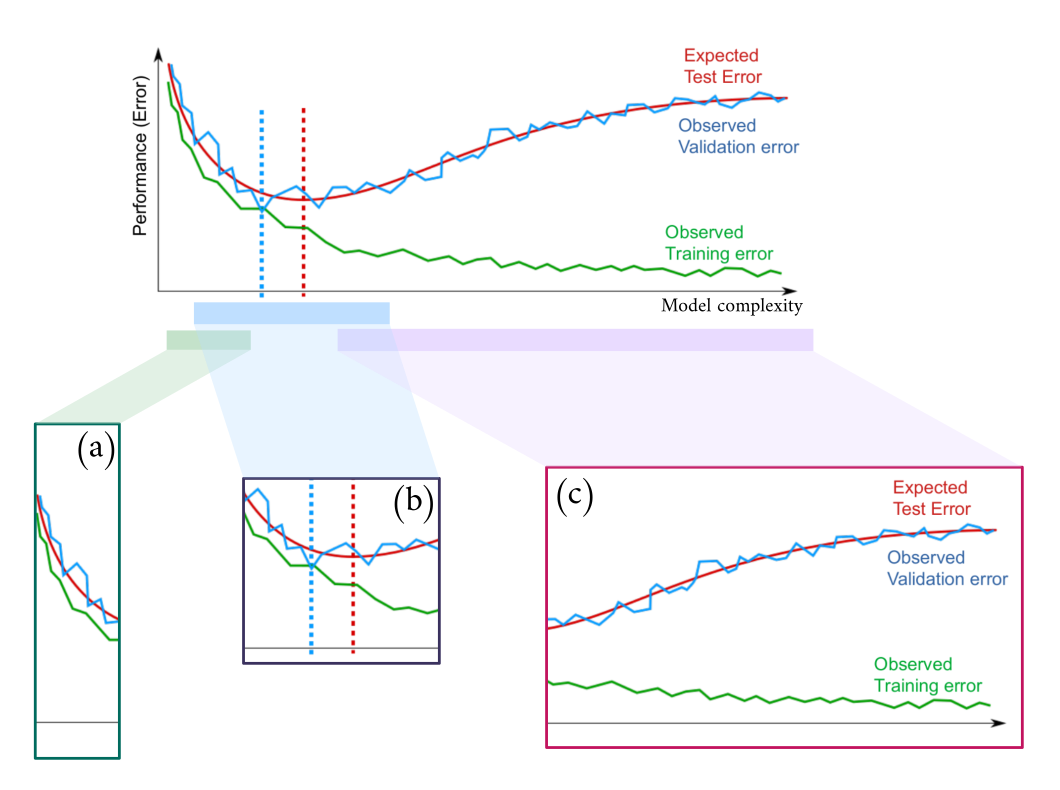
\includegraphics[width=0.8\textwidth]{../ex_train_val_test.png}
\end{figure}

\begin{itemize}
\item[Q1.1] What is the whole figure about?  
\item[A1.1] The figure is showcasing how model complexity effects the model's performance (errors). It tries to explain how increasing the complexity of models reduce observed training error, expected test error, and observed validation error until a certain range (the range with blue and red cut offs) of equilibrium. Then, the more we fit the training data, the more validation error we observe. In conclusion, it shows the side-effect of overfitting the model to our training data. \\

\item[Q1.2] Explain the behaviours of the curves in each of the three highlighted sections in the figure, namely (a), (b), and (c).   
\item[A1.2] Section (a) shows as the model complexity increase, both training and validation (expected test) error decreasing exponentially. Section (b) displays the range where observed training error's decrease becoming much slower even though model complexity increases, while in that range, the expected error and validation error start increasing (on the point where red line stands) as the model complexity increases. In section (c), as the model complexity increases, the expected test error rises like a log function while observed training error slowly converges towards 0 errors.\\

\begin{itemize}
\item[Q1.2.a] Can you identify any signs of overfitting or underfitting in the plot? If yes, explain which sections correspond to which concept.
\item[A1.2.a] Anything after optimal complexity is overfitting and anything before optimal complexity is underfitting, and the point of optimal complexity on the figure would be where the red dotted line is.\\

\item[Q1.2.b] How can you determine the optimal complexity of the model based on the given plot?
\item[A1.2.b] The model optimal complexity is where the red line is. Reason being, it is the minima of expected test error function. In a situation where the observed validation error is unkown and observed training error does not indicate much information regarding optimality of model complexity, this assumption would be the closest standard to the actual optimal complexity. However, if we know the observed validation error, the optimal model complexity will be where the blue dotted verticle line is, as that is where there is least observed validation error is. \\
\end{itemize}
	
\item[Q1.3] Is there any evidence of high approximation risk? Why? If yes, in which of the below subfigures?  
\item[A1.3] Amongst the subfigures, the subfigure (c) would be an evidence of high approximation risk. High approximation risk means a scenario where the model performs well against training data but poorly on test data. In section (c), it shows very little observed training error while the observed validation error being very high and increasing. Hence, by definition of high approximation risk, section (c) is an evidence of it.\\

\item[Q1.4] Do you think that increasing the model complexity can bring the training error to zero? And the structural risk?  
\item[A1.4] Yes, it should theoretically be possible to bring down the training error to zero but bringing the structural risk to zero is practically impossible. Because structural risk is a trade-off between bias and variance of the model which is a pair of competing issues. Fundamentally, if we want to increase the training complexity to 0, we have to increase the complexity but in that case it over-fits to the training data and when it over-fits, it doesn't perform well against unseen data, which reduces generalization factor.\\

\item[Q1.5] If the X axis represented the training iterations instead, would you think that the training procedure that generated the figure used early stopping? Explain why. (\textbf{NB:} ignore the subfigures and the dashed vertical lines)
\item[A1.5] I believe it didn't stop early. If we are assuming the x-axis represented training iteration, the best time to stop the iteration would have been where the minima of expected test error or somewhere approximately there (where the red dotted line is). In fact, the observed validation error and observed training error started to get further apart at this point and it is would be far off the point of where it should have stopped. Hence, it isn't too early point to stop.\\

\end{itemize}

\subsection*{Q2. Linear Regression}
Comment and compare how the (a.) training error, (b.) test error and (c.) coefficients would change in the following cases:
\begin{itemize}
\item[Q2.1] $x_3 = x_1 + 0.2 \cdot x_2$.
\item[A2.1] Important characteristic of the new feature $x_3$ is that it is a linear combination of $x_1$ and $x_2$. The training error most likely decrease because the new feature may capture the additional pattern which were not picked up by $x_1 and x_2$, unless the new feature introduces some noise or redundancy. However, in this particular case, we need to pay attention to linear dependence created between independent variables. As it can be noticed from the oxymoronic statement, this kind of factor makes the estimation of individual effects each coefficients have on the model very difficult, leading to Hence, the coefficients calculated from this sort of relation is very sensitive to unseen data and increase the margin of error for test data while overfiting the model to the training data.\\

\item[Q2.2] $x_3 = x_1 ** 2$ (in Python ** is the "power" operator, so  3 ** 2 = 3 * 3 = 9).
\item[A2.2] By introducing $x_3=x_1**2$, the model is capable of capturing quardratic relationship between $x_1$ and $y$. Naturally, if there is any non-linear relationship, the training error will be reduced. Even if linear, due to $x_1 and x_2$, the training error will not worsen. Similarly, the more flexible quardratic model will capture more complex patterns in the data and reduce test validation error if there is a quardratic relationship. If there is a quardratic relationship, $\theta_3$ will be non-zero and change other $\theta$ values as well, while if there isn't the original $\theta_1, \theta_2$ won't be changed. \\

\item[Q2.3] $x_3$ is a random variable independent from $y$.
\item[A2.3] If $x_3$ is a random variable in the model that is independent from $y$, $\theta_3$ which corresponds to $x_3$ likely to be 0 but if not very close to 0 due to noise in the data. Hence, the $\theta_1, \theta_2$ will have very little to no change due to it. Naturally, as the coefficients of the model not being changed by a significant amount, the training data will be fitted using the existing features $x_1 and x_2$ and will experience maybe a slight improvment in training error if not any. This effect passes onto test errors and it will experience a small to no improvement from the $x_3$ random variable which is independent from $y$.\\

\item[Q2.3] How would your answers change if you were using Lasso Regression?
\item[A2.3] Linear regression minimizes MSE, while lasso regression also adds penalty term in addition to it to encourage sparsity in the coefficient vector to only keep the most important features. In this case, if $x_3$ is a linear combination of $x_1$, and $x_2$, it may be reduced to be reduced to 0 depending how severe the penalty (generalization) term is. Hence, introducing $x_3$ may not improve or worsen the performance using lasso regression. In case of non-linear relationship in the model like ${x_3 = x_1 ^ 2}$, the answer would be the same as in case of linear regression and the performance will depend on existence of quardratic relationship between $x_1$ and $y$. In case of $x_3$ being a random variable independent from $y$, the penalty term will most likely reduce the $\theta_3$ to 0, and there weren't be any change in performance in comparison to previous model.  \\

\item[Q2.4] Explain the motivation behind Ridge and Lasso regression and their principal differences.
\item[A2.4] With linear regression, we have risk of overfitting our model to the training data, which leads to poor performance with the unseen data. To avoid this kind of situation, Ridge and Lasso are commonly used as they both have penalty terms to avoid overfitting but with a different approach. Ridge regression penalizes specifically large $\theta$s (coefficients) and mitigates multicolinearity (when there are highly correlated features) issues, while Lasso regression, as explained before, encourages sparse coeffecient vector. In Ridge, all features are retained while some of them are downweighted to minimize the MSE between predicted and actual target values, but lasso performs automatic feature selection where redundant and irrelevant features are removed.  \\  
\end{itemize}

\subsection*{Q3. Logistic Regression}
\begin{itemize}
\item[Q3.1] What are the main differences between the logistic-regression and the perceptron?
\item[A3.1] Both logistic-regression and the perceptron are linear models specializing in binary classifications. However, logistic-regression uses optimization method such as gradient descent method with loss function to optimize the probabilistic objective function and outputs probability estimation of the object being 0 or 1. While, perceptron tries to find a linear decision boundary by updating the boundary according to misclassified examples (convert it to correct classification). Due to its approach, logistic-regression typically reaches convergence if there isn't any inordinary problem, but it is much more common for perceptron to not reach a convergence because there are cases where the data is not linearly separable. \\

\item[Q3.2] Discuss the major limit they share and how neural networks can solve it.
\item[A3.2] As specified in the first part of the answer, both logistic regression and perceptron are linear models and both of them struggle with learning non-linear patterns existing between input features and target variable. On the otherhand, neural networks can handle non-linear relation between input features and target variable using non-linear activation functions such as sigmoid function at the multiple hidden layer levels. For clarification, an activation function is a function of a node in the neural network that calculates the output of the node from the given input and their weight.\\

\item[Q3.3] What is the role of activation functions in feedforward neural networks.
\item[A3.3] As explained in the previous question, an activation function is like the microprocessor of neural network. There are numerous tasks which require capturing of non-linear relationship between the input and target variable such as image recognition and natural language processing. Activation function embedded in nodes is the one responsible for enabling feedforward neural networks to model complex relation between input features and target variable. It ensures its differentiability so the gradients can be calculated during the training process and be used to update the network parameters through optimization algorithms. In deep neural networks there are scenarios where the gradient of the loss function becomes extremely small with respect to the parameters of neural networks. It is quite common case in deep neural networks with many layers, so it becomes very challenging to train complex models effectively. Hence, activation functions such as ReLU" prevent saturation of activation units (nodes) to improve the stability of convergence of the training process.\\
\end{itemize}
\subsection*{Q4. Consider the regression problem shown in the picture below and answer each point.}

\begin{figure}[htbp] %
    \centering
    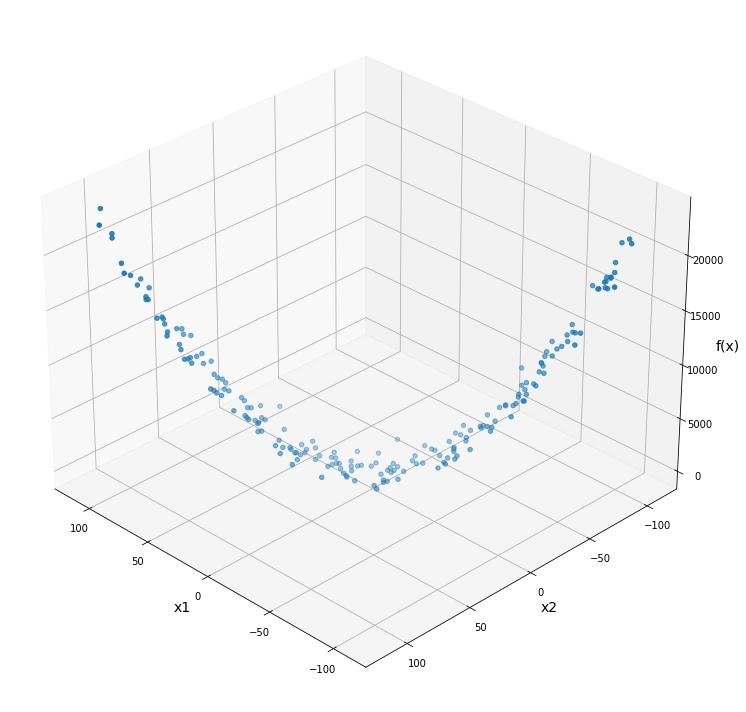
\includegraphics[width=0.7\textwidth]{../parabolic.jpg}
\end{figure}

\begin{itemize}
\item[Q4.1] Do you think a model of the family f(x, theta) = $\theta_0 + \theta_1 * x_1 + \theta_2 * x_2$ is a good choice for such task? Why?

\item [A4.1] First of all, assuming $x_1$, and $x_2$ are linearly independent, the given model is a linear model, whereas we can clearly identify inversed bell-curve on 3D plane, which indicates non-linear relationship between input features and target variable in the picture. As we have numerously iterated in previous questions, a linear model is not sufficient in capturing the non-linear relationship between the input features and the target variable. Hence, it would be much better to use a model capable of capturing non-linear relation such as neural networks or polynomial regression. \\

\item[Q4.2] Do you think using a feed-forward neural network would improve the results?

\item[A4.2] Yes, FFNNs have non-linear activation functions such as sigmoid, ReLU, and more, which in multiple layers would definitely perform better at capturing the non-linear relationship displayed in the picture.

\end{itemize}

\end{document}
